\section{Failure Detection, Tolerance, and Recovery}
\label{sec:fault}


\Fix{Should message failure fall into this section? they seem closely coupled.}
\noindent\textbf{Definition:} 
We need mechanism to detect failures, tolerate failures without impacting the availability of the system, and recover from failures with processing going back to normal.

\Fix{should we discuss failure detection?}

\noindent \textbf{\\Purpose:} 

Failures are the norm. there is a need for a component to detect and recover from failures. since stream jobs are every running jobs, this is an essential component. different modes, provide different guarantees.

\subsection{Failure Detection}
\Fix{maybe talk about heartbeat, pingpong, or piggy back mechanisms?}
\subsection{Failure Tolerance}
\Fix{talk about mechanism used for availability. Maybe the independent design structure that one some of the paths are unavailable not the whole dataflow.}
\subsection{Failure Recovery}

\noindent \textbf{\\Properties:}


	\begin{figure}[h]
	\centering
	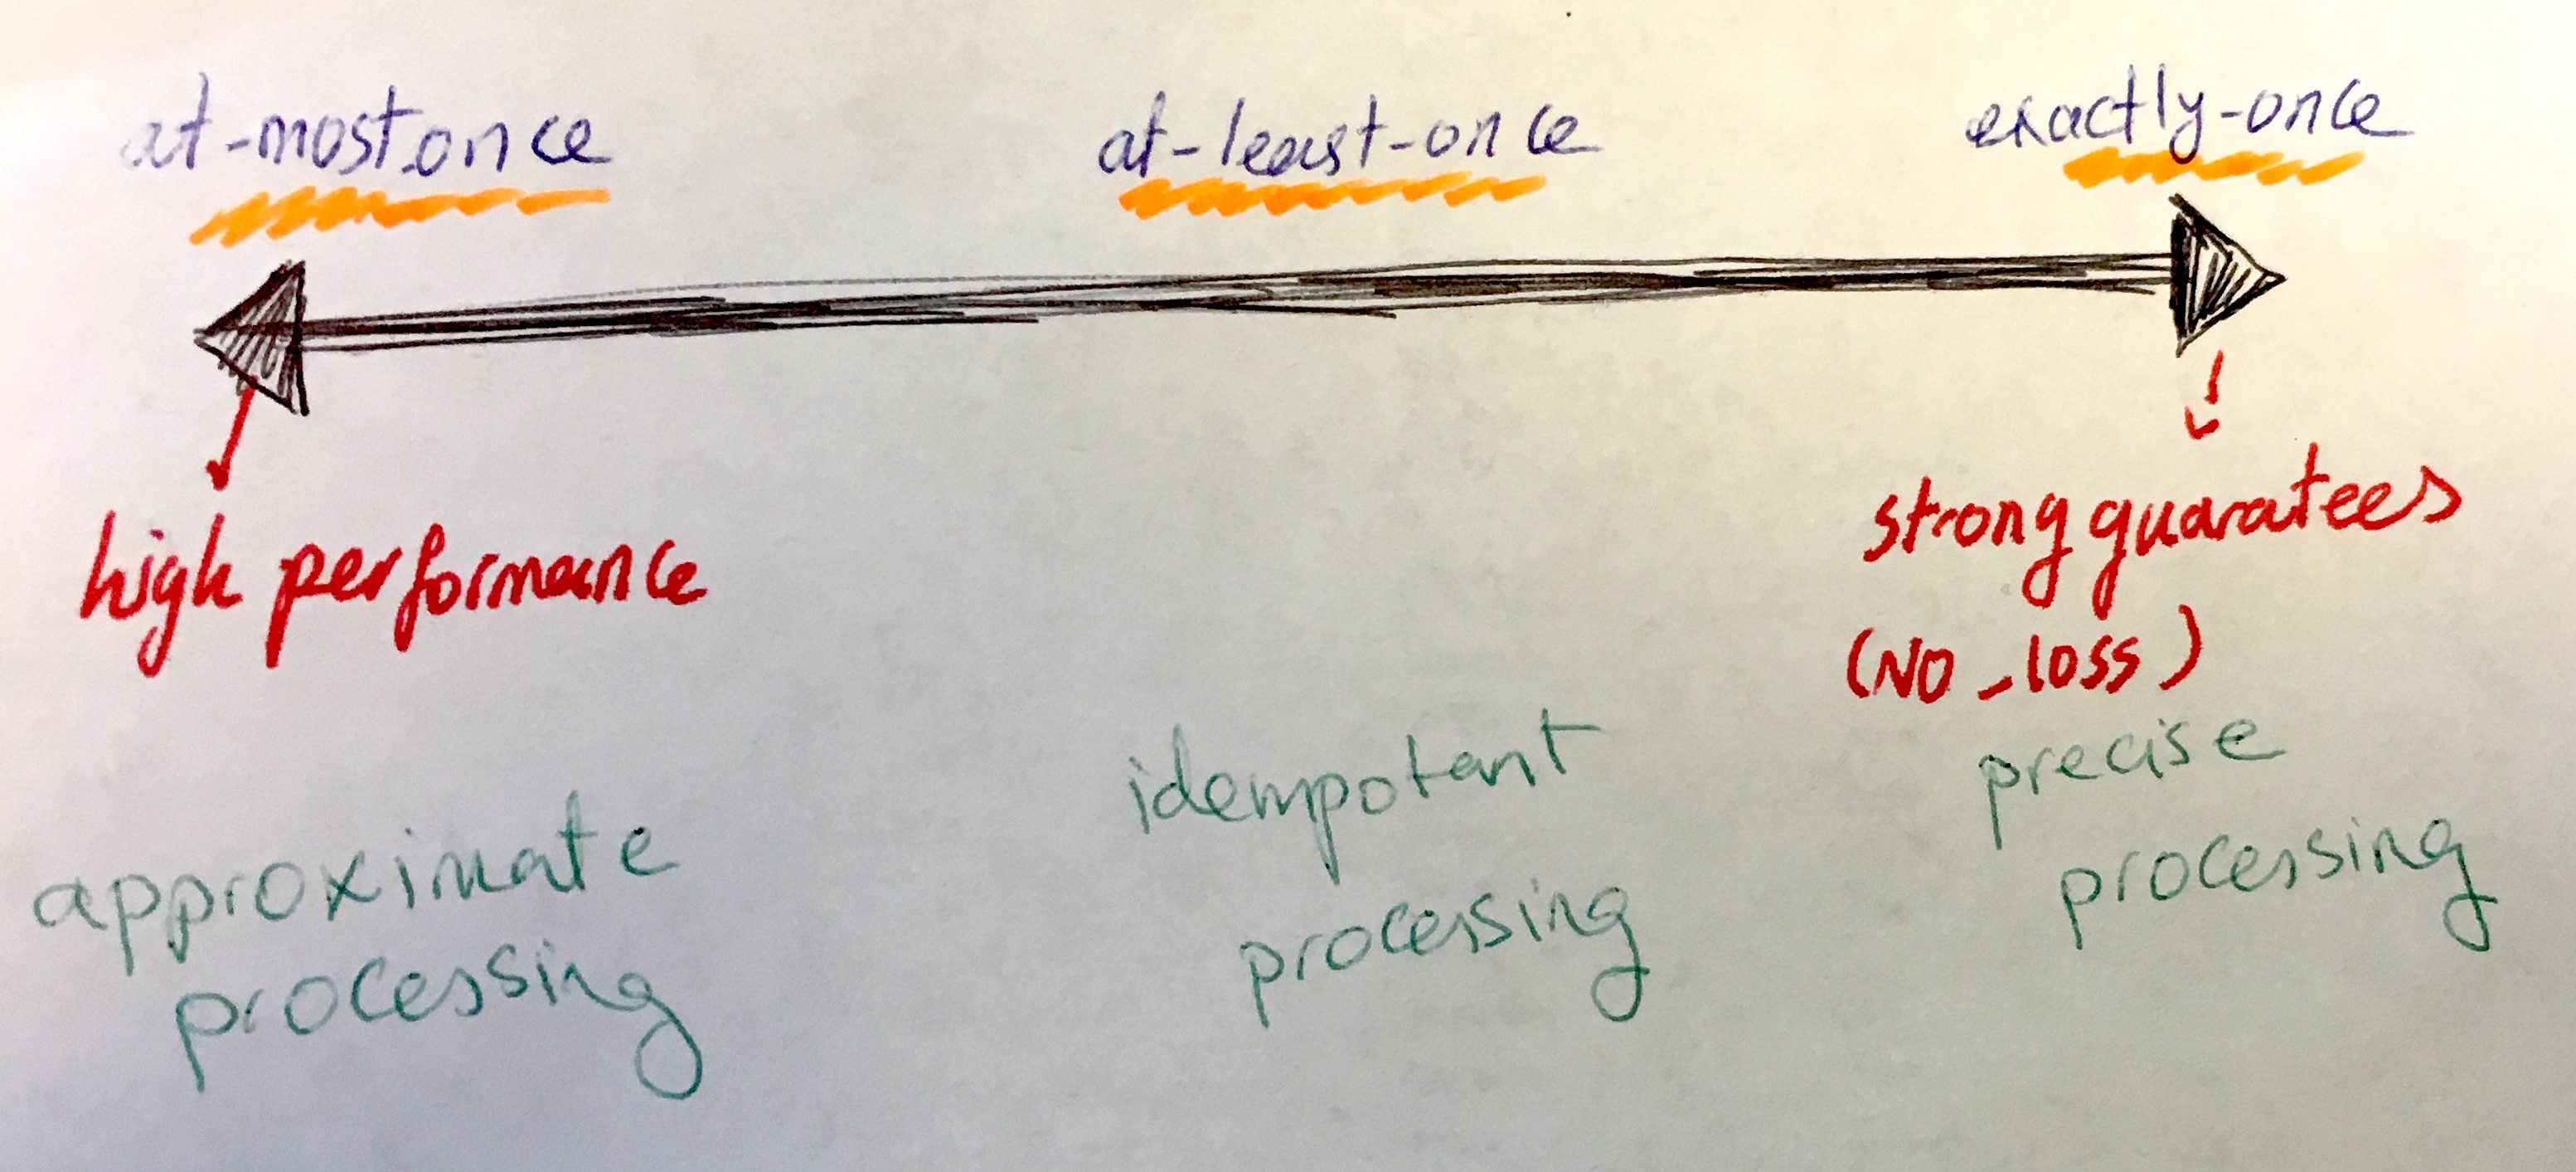
\includegraphics[width=0.45\linewidth]{guarantees.jpg}
	\caption{Spectrum of various failure properties and the trade-off among them.}
	\label{fig:failure}
\end{figure}

	\begin{itemize}
	\item precise recovery:  \borrowed{hides the effects of a failure perfectly, except
		for some transient increase in processing latency, and is
		well-suited for applications that require the post-failure output
		be identical to the output without failure. Many financial
		services applications have such strict correctness requirements.}
	\item rollback recovery: \borrowed{ avoids information loss without guaranteeing
	precise recovery. The output produced after a failure
	is “equivalent” to, but not necessarily the same as, the
	output of an execution without failure. The output may also
	contain duplicate tuples. To avoid information loss, the system
	must preserve all the necessary input data for the backup
	server to rebuild (from its current state) the primary’s state at
	the moment of failure. Rollback recovery is thus appropriate
	for applications that cannot tolerate information loss but
	may tolerate imprecise output caused by the backup server
	reprocessing the input somewhat differently than the primary
	did. Example applications include those that monitor specific
	conditions (e.g., fire alarms, theft prevention through asset
	tracking). We show in Section 6 that this recovery guarantee
	can be provided more efficiently than precise recovery both
	in terms of runtime overhead and recovery speed.}
	\item gap recovery: \borrowed{ our weakest recovery guarantee, addresses
	the needs of applications that operate solely on the most recent
	information (e.g., sensor-based environment monitoring),
	where dropping some old data is tolerable for reduced
	recovery time and runtime overhead}
	\end{itemize}


\noindent \textbf{\\Solutions \& trade-offs:}

\borrowed{ employs a different combination of redundant
	computation, checkpointing, and remote logging, they offer
	different tradeoffs between runtime overhead and recovery
	performance.
}
\begin{itemize}
	\item \borrowed{all following items borrowed!}
	\item amnesia, a lightweight scheme that provides
	\textbf{gap} recovery without any runtime overhead (Section 4).
	\item  passive standby and active standby, two
	process-pairs [4, 10] approaches tailored to stream processing.
	In passive standby, each primary server (a.k.a. node) periodically
	reflects its state updates to its secondary node. In
	active standby, the secondary nodes process all tuples in parallel
	with their primaries. 
	\item  propose upstream backup,
	an approach that significantly reduces runtime overhead compared
	to the standby approaches while trading off a small
	fraction of recovery speed. 
	
	Last two items can be both roll-back and precise recovery.
	
	\Fix{are there other approaches?}
\end{itemize}


\begin{table}[h]
	\tbl{Solutions to \Fix{XXX} and their trade-offs	\label{table:failure-summary}}{
		\tiny		
		\begin{tabular}{p{.15 \linewidth}|p{.3 \linewidth}|p{.3 \linewidth}|p{.1 \linewidth}}%
			
			\hline
			\rowcolor[HTML]{E0E0E0} 
			Solution	&Pros&Cons & Usecase
			\csvreader[head to column names]{tables/template-summary.csv}{}% use head of csv as column names
			{\\\hline\textbf{\csvcoli} & \csvcolii & \csvcoliii & \csvcoliv}% specify your coloumns here
			\\ \hline
		\end{tabular}	
	}
\end{table}


\noindent \textbf{\\Future Direction:}  






